\section{Applying the Premerger Search}
\label{sec:zerolatency_sangria}

Our search uses a zero-latency filter such that data from the future is not required. A full
description is in~\cite{CabournDavies:2024hea}, and is based on work from~\cite{Tsukada:2017cuf}.

We apply this search to the LISA Data Challenge dataset~\cite{Baghi:2022ucj, LDC_WEBSITE}.
The LISA Data Challenges are designed to provide comprehensively modelled data as an introduction
to LISA data analysis. The dataset considered here is Challenge 2a, also known as
\textit{Sangria-HM}~\cite{LDC_WEBSITE_SANGRIA_HM}.
This dataset is similar to Challenge 2: Sangria~\cite{LDC_WEBSITE_SANGRIA, le_jeune_2022_7132178};
it contains exactly the same sources but uses a different waveform model, \texttt{PhenomHM}~\cite{}
... \gscd{A couple of sentences of introduction to sangria - maybe this isnt a subsection?}

To apply this search, we set up the data so that we can truncate it, this was done in hourly intervals,
and then apply the search at 14, 7, 4 and 1 days before merger.

\subsection{Noise Estimation}
\label{subsec:psds}
Our first consideration is to check whether the data from the Sangria dataset has
similar noise properties to the datasets used our previous work. 
\gscd{How does the Sangria dataset compare to the PSDs that we used to set up the zerolatency filter banks?}

\begin{figure*}
    \centering
    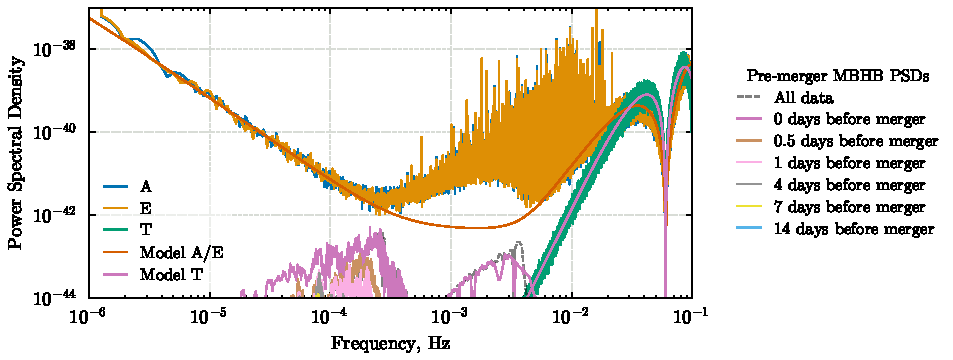
\includegraphics[0.75\textwidth]{images/figure_X_psds_with_premerger_mbhbs.pdf}
    \caption{}
    \label{fig:psds}
\end{figure*}

As a result, we can use the template banks from the zero-latency search paper without significant issues.

\subsection{Secondary Peaks in Signal-to-Noise Ratio}
\label{subsec:double_peaks}
\gscd{Discussion of finding the secondary peaks in the SNR.}

\subsection{Secondary Peak Removal}
\label{subsec:peak_removal}
\gscd{Removing the peaks, and the results of the search including removing the peaks. Discussion of whether assuming that the signal is known is valid or not}

Signal 1 appears to now be missed in the plot, however the former peak in SNR is from the 0.5 days after merger analysis
matching to the peak itself.
Signal 5 can now be seen, as the contamination from the louder Signal 4 is now no longer a problem.

\subsection{Search Results}
\label{subsec:zerolatency_results}
\gscd{Discussion of the analysis results}